\documentclass[a4paper,12pt]{article}

\usepackage{epsf,psfrag,graphicx,color}
\usepackage{hyperref,amssymb}
\usepackage{verbatim}
\usepackage{fancybox}
\usepackage{tcolorbox}

\newcommand{\mybox}[1]{\fcolorbox{black}{blue}{\parbox{\textwidth}{\color{white}#1%
}}}

\definecolor{mycolor}{rgb}{0.122, 0.435, 0.698}% Rule colour
\makeatletter
\newcommand{\myboxx}[1]{%
  \setbox0=\hbox{#1}%
  \setlength{\@tempdima}{\dimexpr\wd0+13pt}%
  \begin{tcolorbox}[colframe=mycolor,boxrule=0.5pt,arc=4pt,
      left=6pt,right=6pt,top=6pt,bottom=6pt,boxsep=0pt,width=\@tempdima]
    #1
  \end{tcolorbox}
}
\makeatother

\definecolor{bt}{rgb}{0.23, 0.55, 0.96}

\newtcbox{\myovalbox}{colback=bt,%
  fontupper=\footnotesize\sffamily\color{white},%
  boxrule=0pt,arc=5pt,%
  boxsep=2pt,left=3pt,right=3pt,top=3pt,bottom=3pt}%

\newcommand{\qchem}{\href{http://q-chem.com}{{\scshape Q-Chem}}}
\newcommand{\iqmol}{\href{http://iqmol.org}{{\scshape IQmol}}}
\newcommand{\symmol}{{\scshape Symmol}}

\newcommand{\heading}[1]{ \noindent{ \large \bf{#1} }}
\newcommand{\myline}{\setlength{\unitlength}{1mm}
                     \begin{picture}(160,2)
                     \put(0,0){\line(1,0){160}}
                     \put(0,1){\line(1,0){160}}
                     \end{picture}
                    }
\newcommand{\showlines}[1]{}

\newcommand{\alert}[1]{\textcolor{red}{#1}}
\newcommand{\sci}[2]{\ensuremath{#1\times 10^{-#2}}}
\newcommand{\mc}{\multicolumn}
\newcommand{\R}[1]{\ensuremath{\mathrm{#1}}}
\newcommand{\B}[1]{\ensuremath{\mathbf{#1}}}

\newcommand{\bt}{\ensuremath{\blacktriangleright}}
\newcommand{\ie}{\emph{i.e.}}
\newcommand{\eg}{\emph{e.g.}}

\setlength{\headheight}{0cm}
\setlength{\topmargin}{1cm}
\setlength{\headsep}{0cm}
\setlength{\voffset}{0cm}
\setlength{\oddsidemargin}{0cm}
\setlength{\evensidemargin}{0cm}
\setlength{\hoffset}{0cm}
\setlength{\textheight}{23.0cm}
\setlength{\textwidth}{16cm}

\setlength{\parindent}{0cm}
\setlength{\parskip}{1em}
\setlength{\unitlength}{1mm}
\usepackage{chngcntr}
\counterwithin{figure}{section}

%\pagestyle{empty}

%----------------------------------------------------------------------%
\begin{document}
%----------------------------------------------------------------------%

\thispagestyle{empty}
\noindent
\myline\\
\begin{center}
{\bf \LARGE Introduction to IQmol}
\end{center}
\myline\\

\vfill

\begin{center}
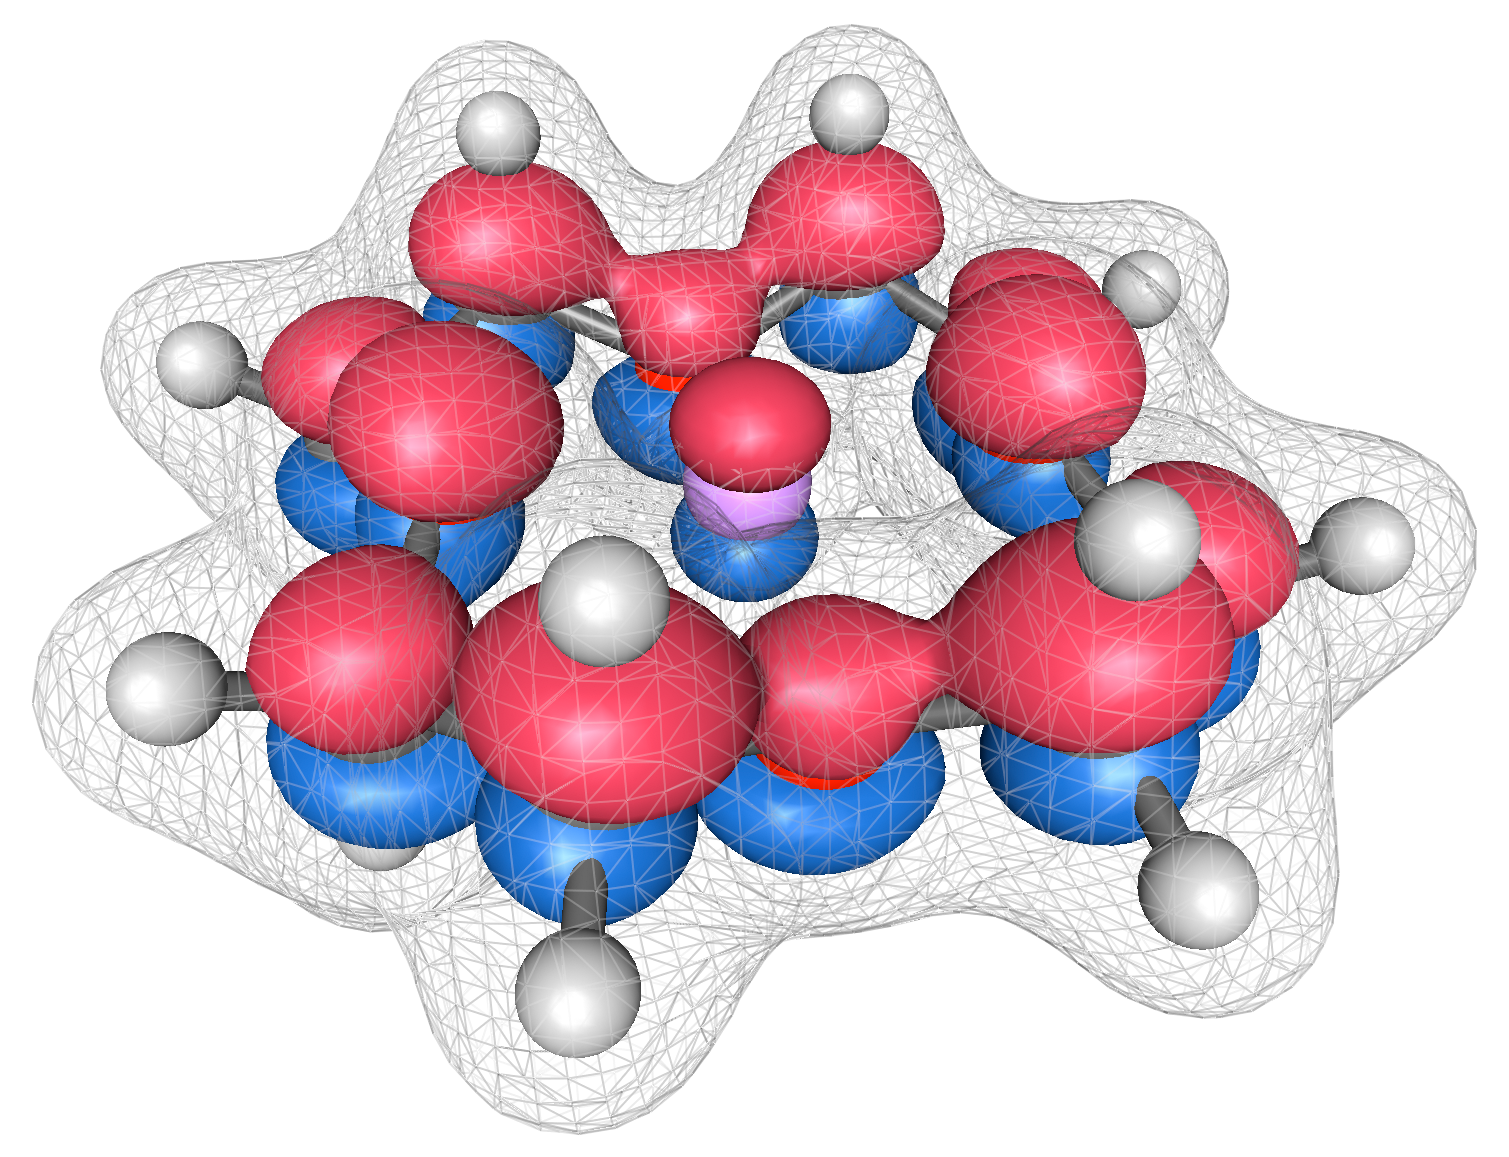
\includegraphics[scale=0.25]{figures/Crown.png}
\end{center}

\vfill
%\myline\\
\begin{center}
{\large v2.9 (2017) Andrew Gilbert}
\end{center}
%\myline\\

\newpage

\tableofcontents

\newpage


%----------------------------------------------------------------------%
\section{Introduction}
%----------------------------------------------------------------------%

\iqmol{} is an open-source molecular editor and visualization package that runs
under Windows, Mac OS X and Linux.  It can read a variety of chemical file
formats including xyz, cml, pdb, mol, fchk, cube data and \qchem{}
input/output.  It also includes a free-form molecular builder that allows
arbitrary molecular structures to be created.  These structures can be
optimized using molecular mechanics force fields and symmetrized to ensure the
structure has the correct point group symmetry.  A library of molecules and
functional groups also exists, and these can be used to facilitate building
more complicated molecules. 

\iqmol{} is capable of displaying a variety of molecular properties including
atomic charges, dipole moments and normal modes.  Several surface types can be
displayed including molecular orbitals, (spin) densities and van der Waals
surfaces. These surfaces can be colored according to an arbitrary scalar field,
such as the electrostatic potential.  Animations are also available for
vibrational frequencies, and reaction and optimization pathways.

\iqmol{} can operate as a stand-alone package, but has also been written to
work seamlessly with the \qchem{} (\url{http://www.q-chem.com}) computational
chemistry package.  A comprehensive input file generator, the \qchem{} User
Interface (QUI), provides access to most of the available options in \qchem{},
and these options are presented in an intuitive, hierarchical fashion.   The
generated input files can be submitted to either local or remote servers that
have the \qchem{} software installed.  In particular, a publicly accessible
server is available that allows small (limited to approximately 10 mins)
quantum chemistry calculations to be run without having to purchase and install
\qchem{}.



\subsection{Installation}

The latest version of \iqmol{} can be downloaded from the website:
\vspace{-1.0em}
\begin{center}
\url{http://iqmol.org/downloads.html}
\end{center}
\vspace{-1.0em}

For Mac (OS X) a disk image file is provided.  After downloading, Simply
double-click the disk image to mount it and copy the application to the
Applications directory, or any other desired location.

For Windows an installer is provided that will guide you through the
installation process and will also create a shortcut to the application on your
desktop.

For Linux .deb and .rpm packages are now available that can be installed using
either dpkg or yum:

\hspace*{2em}{\tt \#>  sudo dpkg -i iqmol\_2.9.0.deb}\\
\hspace*{2em}{\tt \#> sudo apt-get install -f }

The second command is required to resolve the dependency on the Qt libraries,
which you may not have installed.

\hspace*{2em}{\tt \#>  sudo yum install iqmol-2.9.9-2.x86\_64.rpm}

Note that in either case you will need root permission.


\subsection{Overview}
\label{sec:overview}

\begin{figure}[ht]
\begin{center}
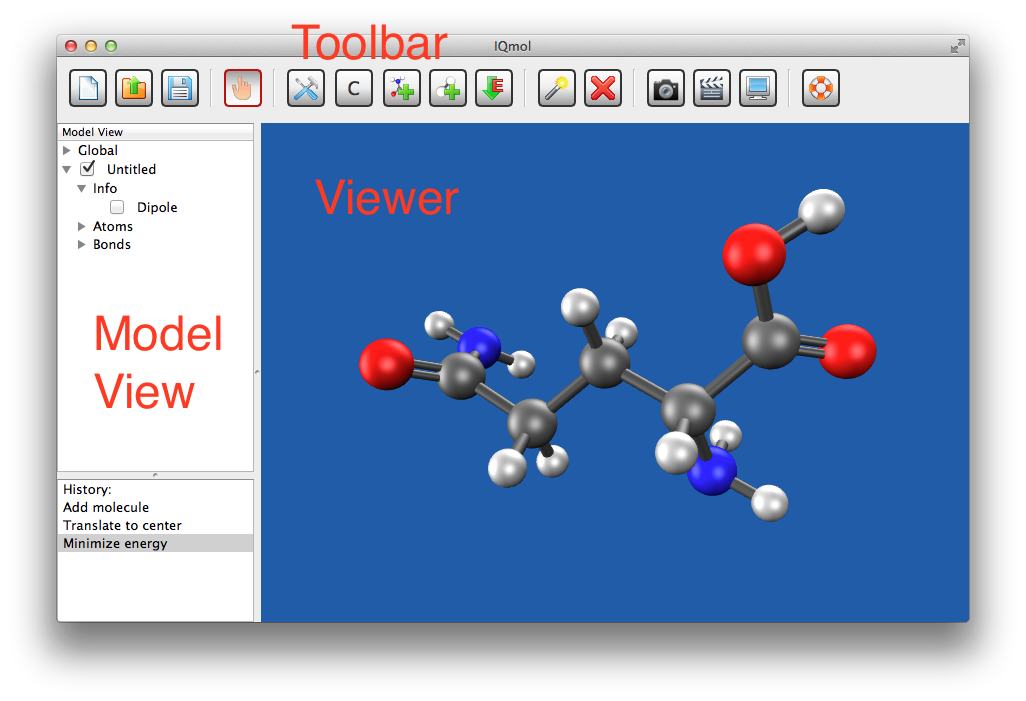
\includegraphics[scale=0.35]{figures/Viewer.png}
\caption{The main \iqmol{} window.}
\label{fig:main}
\end{center}
\end{figure}
The main \iqmol{} window is shown in Fig.~\ref{fig:main} and comprises the
following main parts:
\begin{itemize}
\item The {\bf Viewer} is the main part of the window and is where you can
      view and interact with your molecule.
\item The {\bf Toolbar} at the top provides access to common commands and allows selection
      between different viewer modes including manipulation 
      
\includegraphics[scale=0.40]{figures/ManipulateButton.png}, selection 
      
\includegraphics[scale=0.40]{figures/SelectButton.png} and building.
      
\includegraphics[scale=0.40]{figures/BuildButton.png}
\item The {\bf Model View} panel provides a hierarchical view of the data that
      are available for the molecule.
\item The {\bf History} panel in the lower left shows a list of the most recent
      actions than can be undone, either by clicking on them or by using the
      Edit \bt\ Undo menu option. 
\end{itemize}

The Model View (MV) provides control over what objects are displayed in the Viewer,
and also allows access to configuration options for these objects.  Visibility is
controlled by the associated check-box.  Unchecking a check-box causes the item
and all its children to become hidden.  If an item does not have a check-box,
for example a bond, then its visibility can only be controlled by items higher
in the hierarchy.  

The appearance of many objects can be configured by double-clicking the item in
the MV.  For example, double-clicking the molecule name brings up the Configure
Molecule dialog which allows you to change the appearance of the molecular
structure:
\begin{center}
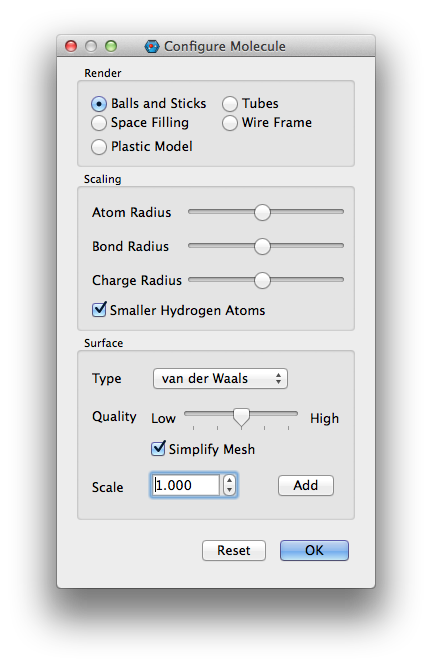
\includegraphics[scale=0.25]{figures/MoleculeConfigurator.png}
\end{center}
Note that several molecules can be viewed concurrently in the same Viewer
and the appearance of each can be configured separately.  
\begin{figure}[h]
\begin{center}
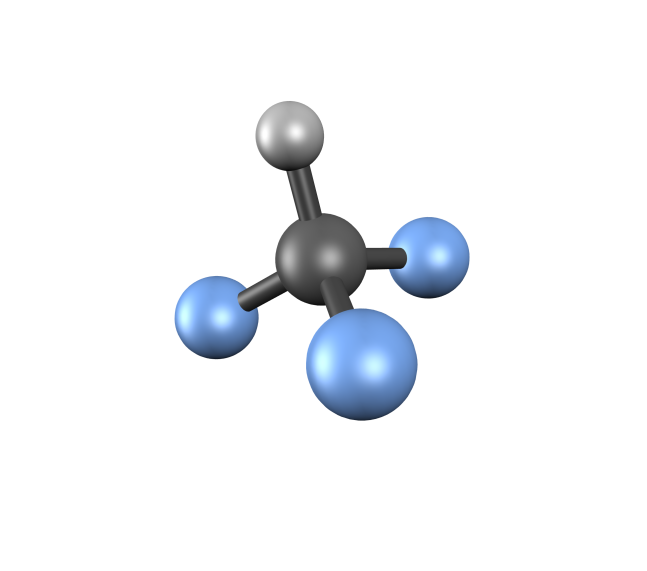
\includegraphics[scale=0.18]{figures/CHF3-balls.png}\hspace{-3mm}~
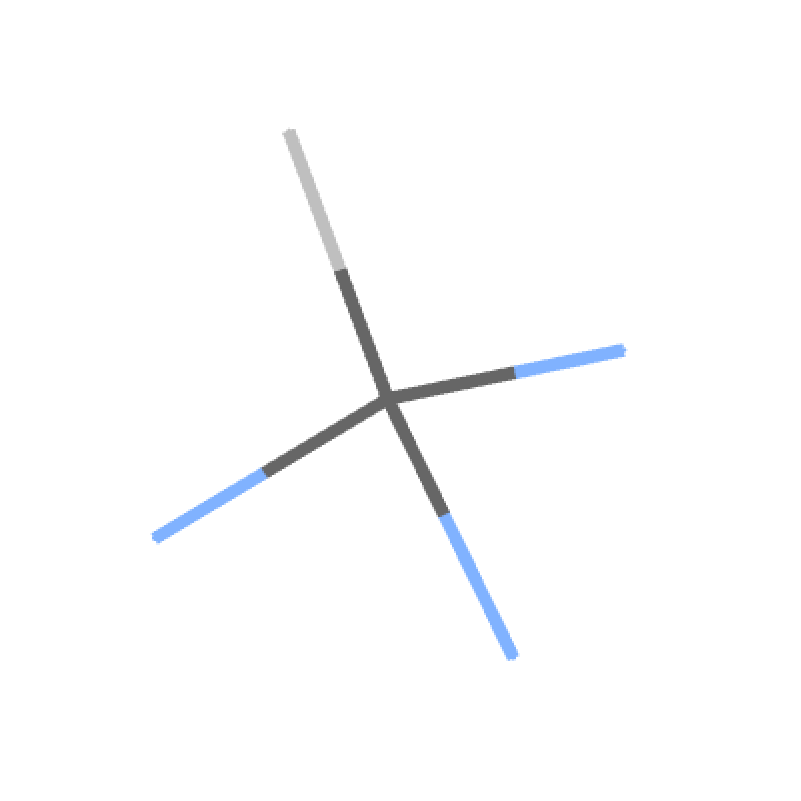
\includegraphics[scale=0.20]{figures/CHF3-wire.png}\hspace{-3mm}~
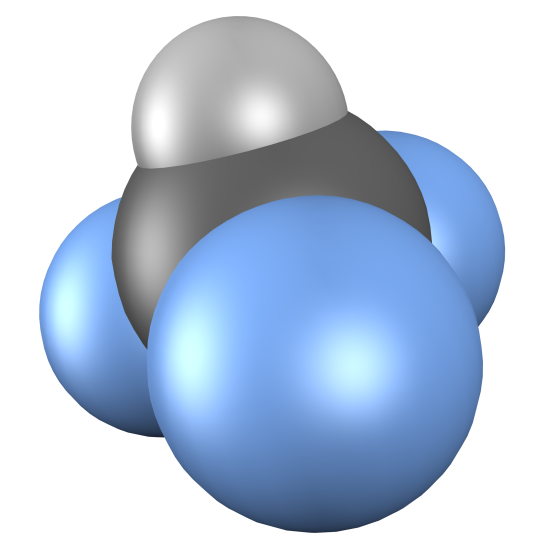
\includegraphics[scale=0.18]{figures/CHF3-space.png}\hspace{-3mm}~
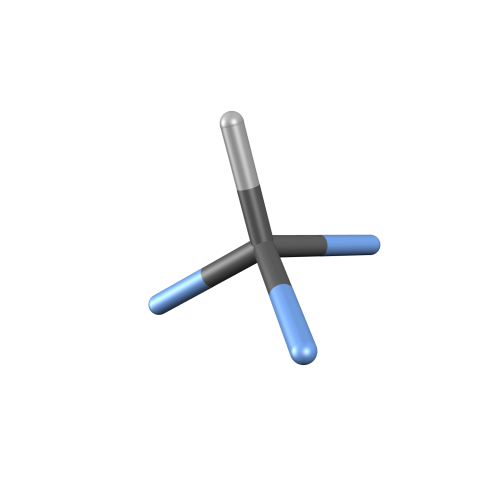
\includegraphics[scale=0.18]{figures/CHF3-tubes.png}\hspace{-3mm}~
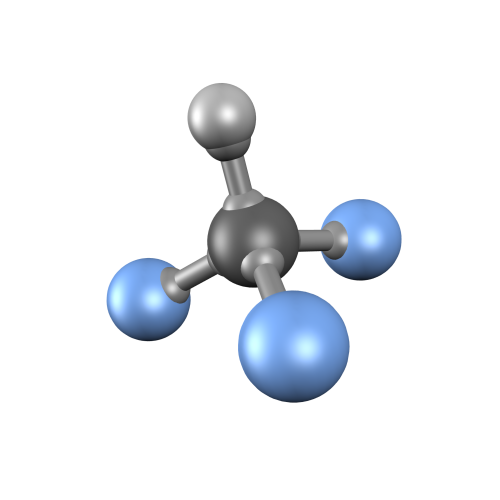
\includegraphics[scale=0.18]{figures/CHF3-moly.png}
\caption{Rendering styles for molecular structures: balls and sticks, wire frame,
space filling, tubes and plastic.}
\label{fig:styles}
\end{center}
\end{figure}



%----------------------------------------------------------------------%
\newpage
\section{Building Molecules}
%----------------------------------------------------------------------%


\subsection{Adding Atoms and Fragments}

By default, \iqmol{} opens in build mode.  This is indicated by a red border
around the 
\includegraphics[scale=0.40]{figures/BuildButton.png} button in the
Toolbar.   The default build atom is indicated by the

\includegraphics[scale=0.40]{figures/BuildAtomButton.png} button and can be changed
by clicking on this button.  A pop-up periodic table will appear from which the
desired element type can be selected.

Clicking in the empty Viewer window will create an atom of the current build
element. Additional atoms can be added by clicking on an existing atom and
dragging the mouse.  This creates a new atom bonded to the first.  To create a
disconnected atom, hold down the \emph{alt} modifier key when clicking in the
Viewer window.  (Note that some Linux window managers use the \emph{alt} modifier
for other purposes.  This behavior can be changed using System Settings 
\bt\ Keyboard \bt\ Short-cuts menu).

Bond orders can be increased by clicking and dragging between two existing
atoms.  If no bond exists between the two atoms,  one is created.  Otherwise
the bond order is increased.  To decrease the bond order, the bond must first
be deleted and a new bond created.
\begin{figure}[h]
\begin{center}
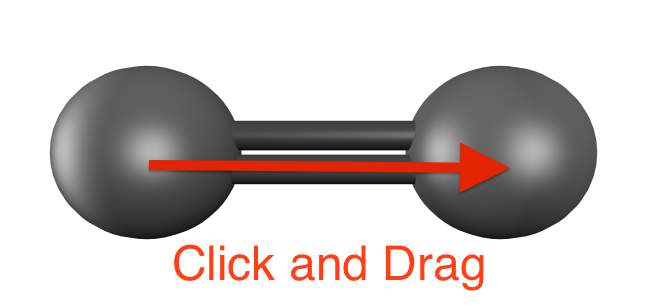
\includegraphics[scale=0.25]{figures/Cdouble.png}
\caption{Increasing the bond order.}
\end{center}
\end{figure}


Functional groups can be added by clicking the

\includegraphics[scale=0.40]{figures/BuildFragButton.png} button, ensuring the
Functional Group radio button is clicked and selecting the desired group from
the menu.  Groups are added in the same way as atoms, \emph{i.e.} clicking and
dragging from an existing atom.  The empty valence is indicated by the yellow
bond and shows where the group will be connected.
\begin{figure}
\begin{center}
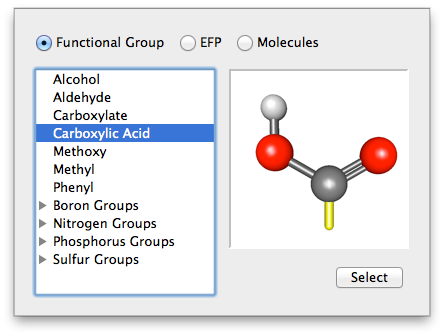
\includegraphics[scale=0.5]{figures/FunctionalGroup.png}
\caption{The build fragment pop-up that appears when the add fragment button
is clicked.} 
\end{center}
\end{figure}


Entire molecules can also be added to your system by clicking the

\includegraphics[scale=0.40]{figures/BuildFragButton.png} button, ensuring the
Molecules radio button is clicked, and selecting the desired molecule from the
menu.  Be sure to click \Ovalbox{Select} or the build selection will not be
updated.  Unlike the other build modes, clicking anywhere in the viewer window
will add the selected molecule (no mouse modifier is required).  This allows
several molecules of the same type to be added quickly, (\eg\ for
solvation), but changes the usual mouse behavior.  If you accidentally add too
many molecules, use the Edit \bt\ Undo menu option.  When adding molecules, if
you click and hold it is possible to alter the local orientation of the newly
added molecule before being added to the global frame.
%\begin{center}
%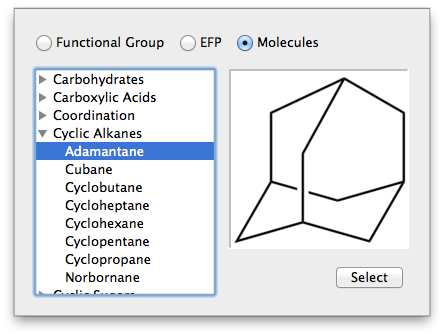
\includegraphics[scale=0.5]{figures/BuildMol.png}
%\end{center}

Once the backbone of the molecule has been drawn, the Add Hydrogens button

\includegraphics[scale=0.40]{figures/AddHydrogensButton.png} can be clicked to
automatically add hydrogen atoms to any unfilled valencies.



\subsection{Optimizing Structures Using Molecular Mechanics}

The builder in \iqmol{} is free-form, so your initial structure may look a bit
wonky.  To improve the geometry, click the

\includegraphics[scale=0.40]{figures/MinimizeEnergyButton.png} button.  This
optimizes the geometry using a molecular mechanics (MM) force field.   The
default force field is the Universal Force Field (UFF)\cite{UFF} which has the
advantage of being defined for almost all of the periodic table.  However, the
UFF does not perform well for systems that contain hydrogen bonds and, in these
cases, it is recommended that the force field be changed using the Build \bt\
Select Force Field menu option.

\begin{figure}[h]
\begin{center}
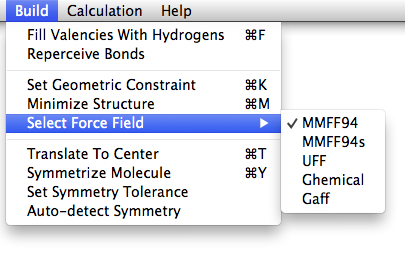
\includegraphics[scale=0.5]{figures/ForceFieldMenu.png}
\caption{Changing the molecular mechanics force field.}
\end{center}
\end{figure}


\subsection{Symmetrizing Structures}

If your molecule has symmetry, the MM optimization is unlikely to find a
structure with the desired symmetry.  If this is the case, a nearly symmetric
structure can be symmetrized using the Build \bt\ Symmetrize
Molecule menu option.  Finding very high symmetry may require relaxing the
tolerance using the Build \bt\ Set Symmetry Tolerance menu
option.  Relaxing the tolerance allows the program to move the nuclear
coordinates more in order to find a symmetric structure.

\iqmol{} uses a modified version of the \symmol{}\cite{SymMol} program written
by Tullio Pilati and Alessandra Forni to symmetrize molecular structures.



\subsection{Specifying Geometric Parameters}

Specific values for geometric parameters can be set by first selecting the
atoms involved and using the Build \bt\ Set Geometric Constraint menu
option.  A dialog will appear that allows the parameter to be either set,
constrained or scanned.  Constrained parameters apply to any subsequent MM
optimization and are also passed through to the \qchem{} input file, if a
optimization job is requested.  Scan options are also passed through to
\qchem{} for scan jobs.

\begin{figure}[h]
\begin{center}
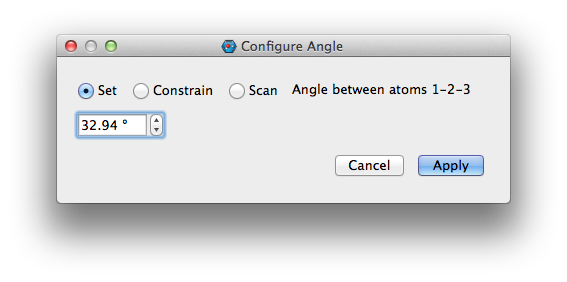
\includegraphics[scale=0.5]{figures/ConstraintDialog.png}
\caption{Dialog for setting geometric constraints}
\end{center}
\end{figure}

The type of constraint depends on the number of atoms selected:
\vspace{-1em}
\begin{enumerate}
\itemsep0em
\item Fixed atom position
\item Inter-atomic distance (or select a single bond)
\item Bond angle
\item Torsion (dihedral) angle
\end{enumerate}
Active constraints are visible in the Viewer and can be deactivated by clicking
the adjacent check-box in the MV.


\subsection{Manipulating and Selecting Molecules}
\label{sec:mousemodes}

\iqmol{} has been designed to work best with a three-button mouse or track pad.
If you are using a track pad on a  Mac, it is recommended that you enable the
secondary click by going to System Preferences \bt\ Trackpad.

Manipulate mode is activated by clicking the

\includegraphics[scale=0.40]{figures/ManipulateButton.png} button in the
Toolbar, and implements the following mouse functionality:
\begin{itemize}
\item {\bf Left click and drag:} Rotate the view of the molecule.  
\item {\bf Middle click and drag:} Zoom in and out.  
\item {\bf Right click and drag:} Translate the view of the molecule.
\end{itemize}

It is also possible to manipulate part of the molecule independently from the
rest.  To do this, make a selection and press and hold the \emph{ctrl} modifier
(\emph{command} key on Mac).  The mouse movements will affect only the 
selected atoms as follows:
\begin{itemize}
\item {\bf Left click and drag:} Rotate the selected atoms about their center. 
\item {\bf Right click and drag:} Translate the selected atoms.  
\end{itemize}
If only a single bond is selected, then the mouse movements have the following effects
\begin{itemize}
\item {\bf Left click and drag:} Rotate around the axis of the bond.
\item {\bf Right click and drag:} Change the length of the bond.
\end{itemize}

Select mode is activated by clicking the

\includegraphics[scale=0.40]{figures/SelectButton.png} button in the Toolbar,
and implements the following mouse functionality:
\begin{itemize}
\item {\bf Left click:} Adds atom or bond to selection. 
\item {\bf Click and drag:} Creates a selection rectangle, all atoms and bonds
           within the selection rectangle are added to the selection. 
\item {\bf Right click:}  Removes atom or bond from selection.
\end{itemize}
It is also possible to select all, select none and invert the selection via
the options under the Edit menu.


\subsection{Adding Additional Conformers}

For setting up jobs that use the Freezing String Method (FSM), two conformers
are required corresponding to the initial and final geometries of the string.
Having built the first geometry, a second geometry can be added to the molecule
by right-clicking the molecule name in the MV.  This brings up a context menu
with the option `Duplicate Geometry'.  
\begin{figure}[h]
\begin{center}
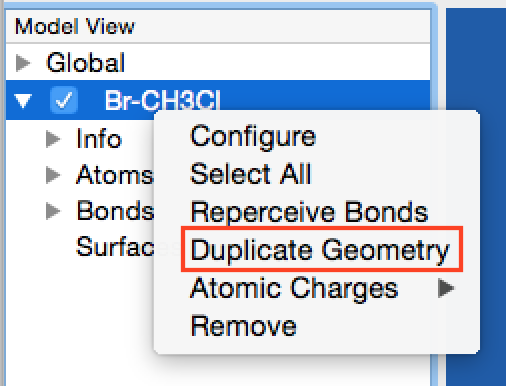
\includegraphics[scale=0.4]{figures/MoleculeContext.png}
\end{center}
\end{figure}
Selecting this menu option creates a Geometries item in the MV with two
(identical) geometries.  The second of these can be modified by selecting it in
the MV and manipulating selected atoms in the viewer using the \emph{ctrl}
(\emph{command} on Mac) modifier key.  If `Freezing String' is chosen for the Calculate
option in the QUI (see the next section) then both geometries will be included
in the \$molecule section of the input deck, separated by ****.





%----------------------------------------------------------------------%
\newpage
\section{Running \qchem{} Calculations}
%----------------------------------------------------------------------%

\subsection{The QUI}

\iqmol{} has a built-in input file generator for \qchem{} calculations, the
QUI, that can be accessed via the Calculation \bt\  Q-Chem Setup menu.  
\begin{figure}[h]
\begin{center}
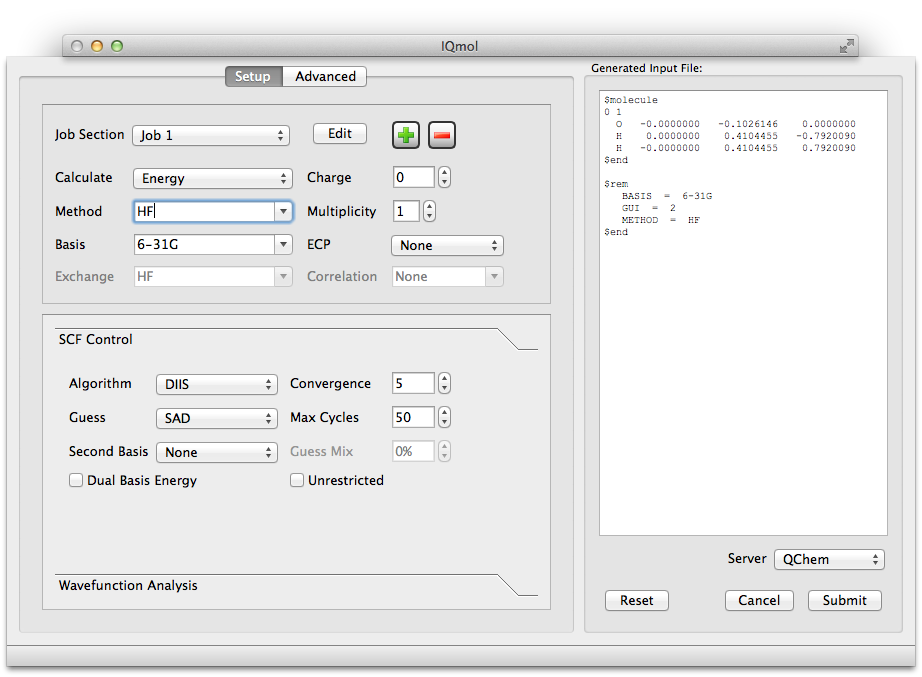
\includegraphics[scale=0.4]{figures/QUI.png}
\caption{The \qchem{} User Interface (QUI) dialog.}
\end{center}
\end{figure}

The left hand side of the QUI dialog contains controls for setting up the
calculation.  These are presented in a hierarchical fashion so that most
commonly used options are presented in the top part of the panel, with other
relevant options appearing in the lower section depending on what type of job
is selected.  More advanced options can be accessed via the Advanced tab.  The
generated input file is echoed in the panel on the right hand side of the QUI.

Clicking the Submit button will start the job running on the selected server.
Once the job has completed you will be prompted to copy the results (for remote
servers) before they are automatically loaded into \iqmol{}.  The

\includegraphics[scale=0.6]{figures/Favourites.png} icon appears next to the
molecule name in the MV when the molecule has been updated with the
results of a calculation.


\subsection{The Job Monitor}

Submitted jobs can be monitored via the Calculation \bt\ Job Monitor menu
option.  This brings up the Job Monitor dialog that provides information on the
progress of jobs.  Right-clicking a row in the Job Monitor brings up a context
menu which allows running jobs to be killed or queried, and finished jobs to be
opened.
\begin{figure}
\begin{center}
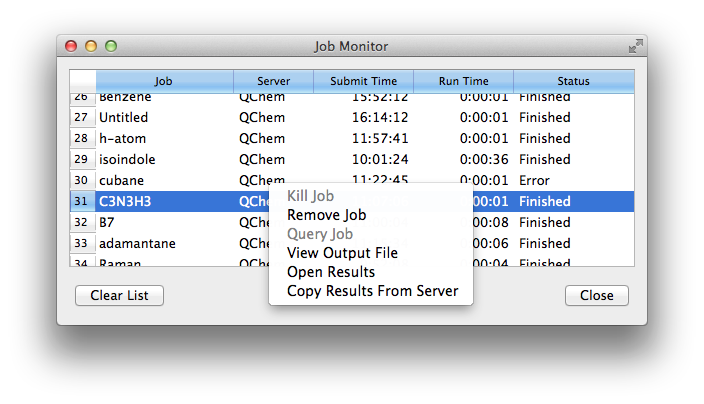
\includegraphics[scale=0.5]{figures/JobMonitor.png} 
\caption{The Job Monitor dialog.  Right-clicking on a selected job brings up
a context menu with additional options.}
\end{center}
\end{figure}

If a job has the Error status, hovering the mouse over the status will show the
error message.  Alternatively, double clicking the job will open the output
file, if available, and may provide additional information about why the job
failed.  Double-clicking a completed job will copy the results from the
server (if they have not already been copied) and reload them into the main
\iqmol{} window.


\subsection{Configuring Servers}

By default \iqmol{} is configured to submit jobs to the \qchem{} server in
Pleasanton, California.  This is a publicly available server than can be used
by anyone wishing to run test calculations before purchasing the \qchem{}
software.  Jobs submitted to this server can access the full suite of
electronic structure methods available in \qchem{}, but are time-limited to 10
minutes. 

Additional servers can be configured to access other computers that have the
\qchem{} software installed.  These computers can be either local servers
(\emph{i.e.} the same machine as the one running \iqmol{}) or remote servers
that can be connected to via SSH.  To add an additional server, go to the
Calculation \bt\ Edit Servers menu option and click the

\includegraphics[scale=0.40]{figures/PlusButton.png} button.  
\begin{figure}
\begin{center}
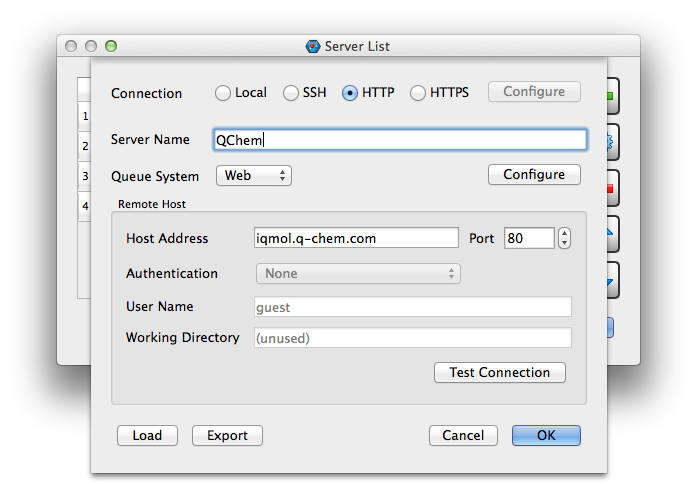
\includegraphics[scale=0.5]{figures/ServerDialog.png}
\caption{The server configuration dialog.}
\end{center}
\end{figure}

The information required to configure a server depends on its type, but default
options exist for each case.  The following indicates the minimum that should
be considered:

\begin{itemize}
\item {\bf Local:} Set the Queue System to `Basic'
      unless you know you are running queuing software on the machine.
      Be sure the {\tt QC} and {\tt QCSCRATCH} variables are set to their correct
	  values in the Run File Template, which is accessed by clicking the Configure
      button.
\item {\bf SSH:} The host name and account on the target machine will 
      be required in order to connect via SSH.  Set the Authentication combo-box to
      `Password Prompt' unless you have set up an alternative authentication protocol.
	  Depending on how the target host has been set up, the Run File Template
	  may require some editing to get it to work, but this will differ from
      machine to machine.
\item {\bf HTTP:} The default options should be suitable.  Note that on Windows
	  HTTP should be used (and is the default in v2.8) whereas for Mac and
      Linux HTTPS can be used and will be the default in future versions.  
\end{itemize}


%----------------------------------------------------------------------%
\newpage
\section{Analyzing Results}
\label{sec:anal}
%----------------------------------------------------------------------%

\iqmol{} reads in a wide variety of file types and allows the user to visualize
many of the results they contain.  Individual files can be opened via the File
\bt\ Open menu option, or alternatively by dragging and dropping the file onto
the Viewer window.  Directories can also be opened via the File \bt\ Open Dir
menu option, or by dragging and dropping the directory onto the Viewer.  

Opening directories allows more than one file associated with a molecule to be
loaded together, such as a \qchem{} output file and a formatted checkpoint
file.  The directory name determines the base name for the molecule and
\iqmol{} loads all files contained within the directory that have a matching
base name.  
\begin{figure}[h]
\begin{center}
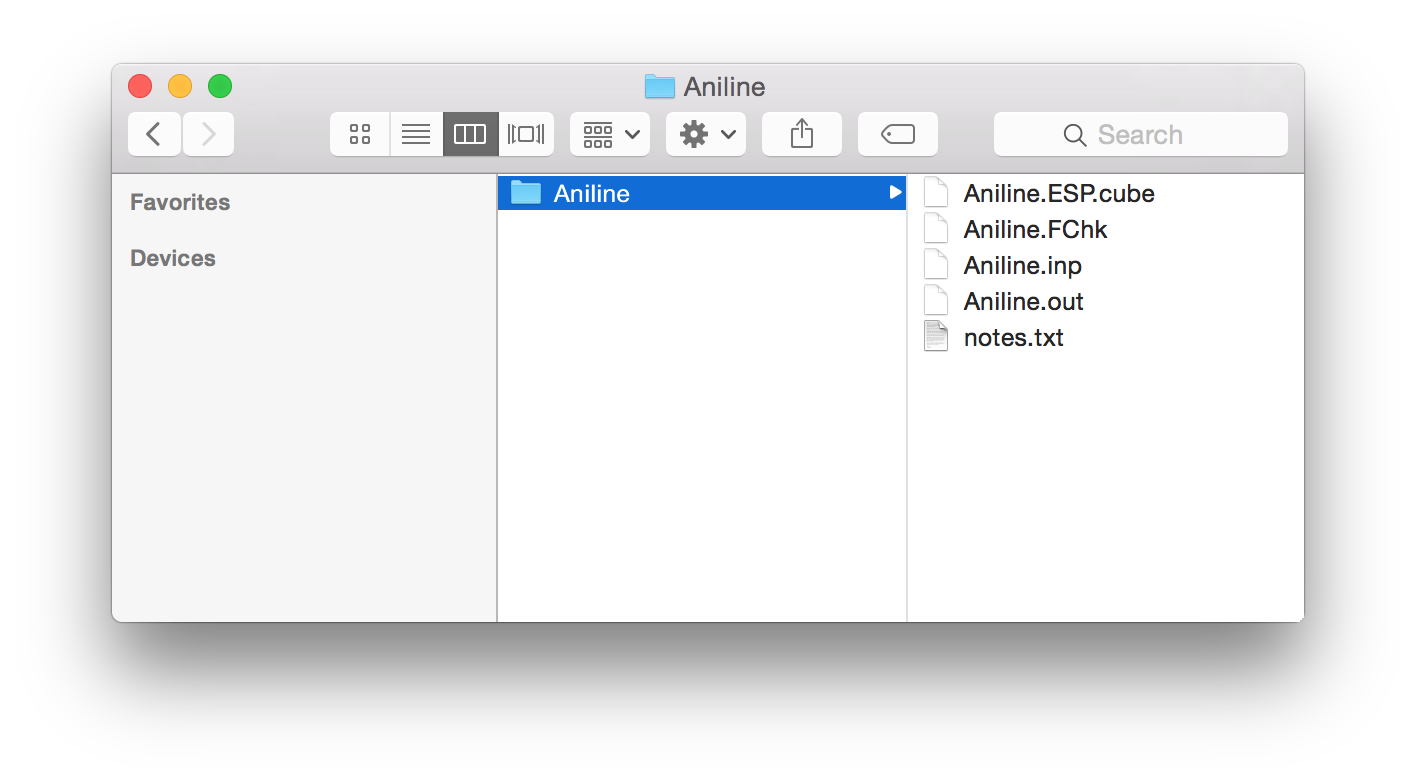
\includegraphics[scale=0.40]{figures/OpenDir.png}
\caption{Example: Opening the Aniline directory will load the Aniline.ESP.cube,
Aniline.FChk, Aniline.inp and Aniline.out files into the one molecule in the
MV.  The notes.txt file will be ignored as it has a different base name.} 
\end{center}
\end{figure}


\subsection{Molecular Surfaces}

Several molecular surfaces can be generated without first performing a quantum
chemical calculation. These include: van der Waals, pro-molecule and
superposition of ionic densities (SID).  The SID surface is similar to the
pro-molecule surface except that it scales the densities based on the atomic
charges of the atoms and may provide a more accurate representation of the
density of charged systems.

To plot one of these pseudo-density surfaces, double-click the `Surfaces'
item in the MV associated with the molecule.




\subsection{Plotting Molecular Orbitals From a Checkpoint File}

\label{sec:mos}
Plotting molecular orbitals (MOs) requires a formatted checkpoint file (.fchk
file extension) which is generated by default when running \qchem{}
calculations from \iqmol{} (GUI rem variable should be set to 2).  After
opening the fchk file, a `Canonical Orbitals' item will appear in the MV under
the Surfaces item.
Double-clicking this brings up the Add Surface dialog:
\begin{figure}[h]
\begin{center}
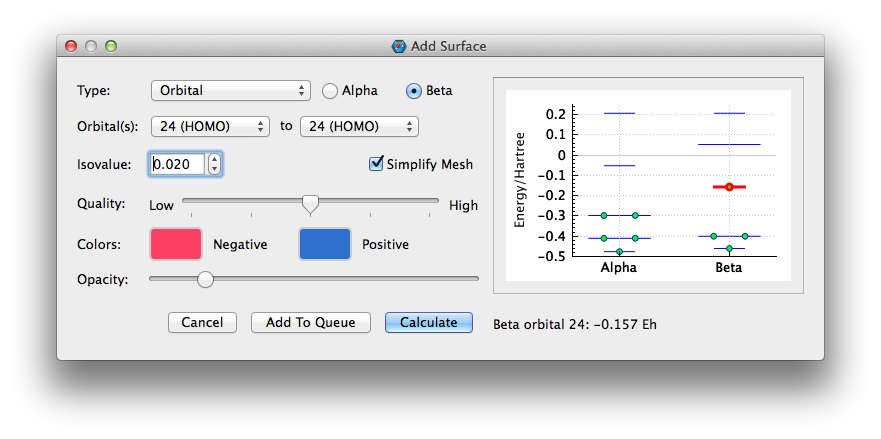
\includegraphics[scale=0.25]{figures/MolecularOrbitalsConfigurator.png}
\caption{The Add Surface dialog allows MOs and (spin-)densities to be plotted.
%The right-hand panel also offers an interactive MO diagram showing occupied and
%virtual orbital energies.
} 
\label{fig:addsurface}
\end{center}
\end{figure}

The Add Surface dialog allows MOs, total densities, and spin densities  to be
computed.  Several surfaces can be queued and computed at the same time, which
is more efficient as the shell data only need to be computed once.  The
quality, colors and opacity of the surfaces can be be set in the dialog, and
changes to these settings are saved to the preferences as default values for
any subsequent surfaces generated.

Note that each tick on the quality scale corresponds to roughly four times the
number of grid points as the previous one, and will therefore take roughly four
times as long to compute.  Also note that densities require evaluating
shell-pair values and are significantly more expensive to compute that MOs,
which only require shell values.  For most purposes, the pseudo densities (such
as the pro-molecule density) available by double-clicking the Surfaces item
provide an almost identical density surface, but at a much cheaper cost.

\begin{figure}[h]
\begin{center}
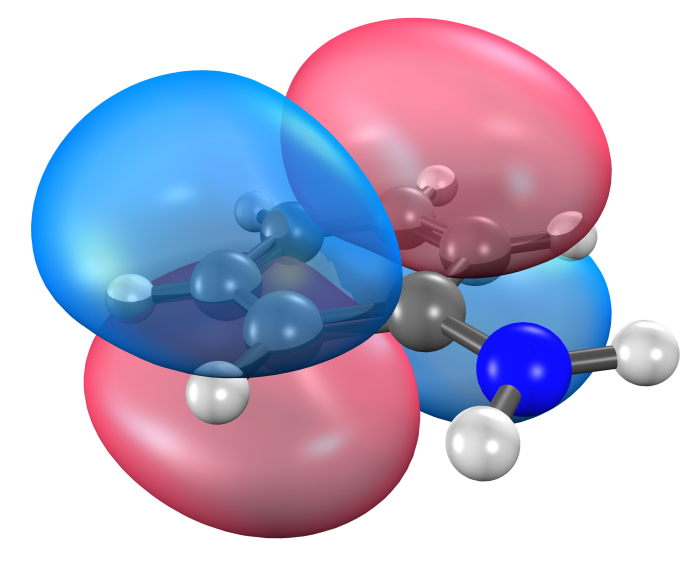
\includegraphics[scale=0.32]{figures/Orbital.png}
\caption{An example molecular orbital for aniline.}
\label{fig:mo}
\end{center}
\end{figure}

Once computed, the individual surfaces appear as sub-items in the MV, and these
can be further configured by double-clicking the item in the MV.

The Add Surface dialog also contains an interactive energy level diagram on the
right-hand side panel.  The vertical scale can be zoomed in and out using the
scroll wheel (or equivalent) on the mouse.  The scale can also be translated by
a left click-and-drag.  Individual orbitals can be selected with a left-click
and this will cause the energy of the selected orbital to appear below the
diagram, as shown in Fig.~\ref{fig:addsurface}.


\subsection{Other Orbitals and Densities}

Orbitals and densities other than those based on the canonical orbitals can
also be visualized, if the appropriate calculation has been performed.  Localized
orbitals, natural transition orbitals, natural bond orbitals and
attachment/detachment densities are all possible.

\begin{figure}[h]
\begin{center}
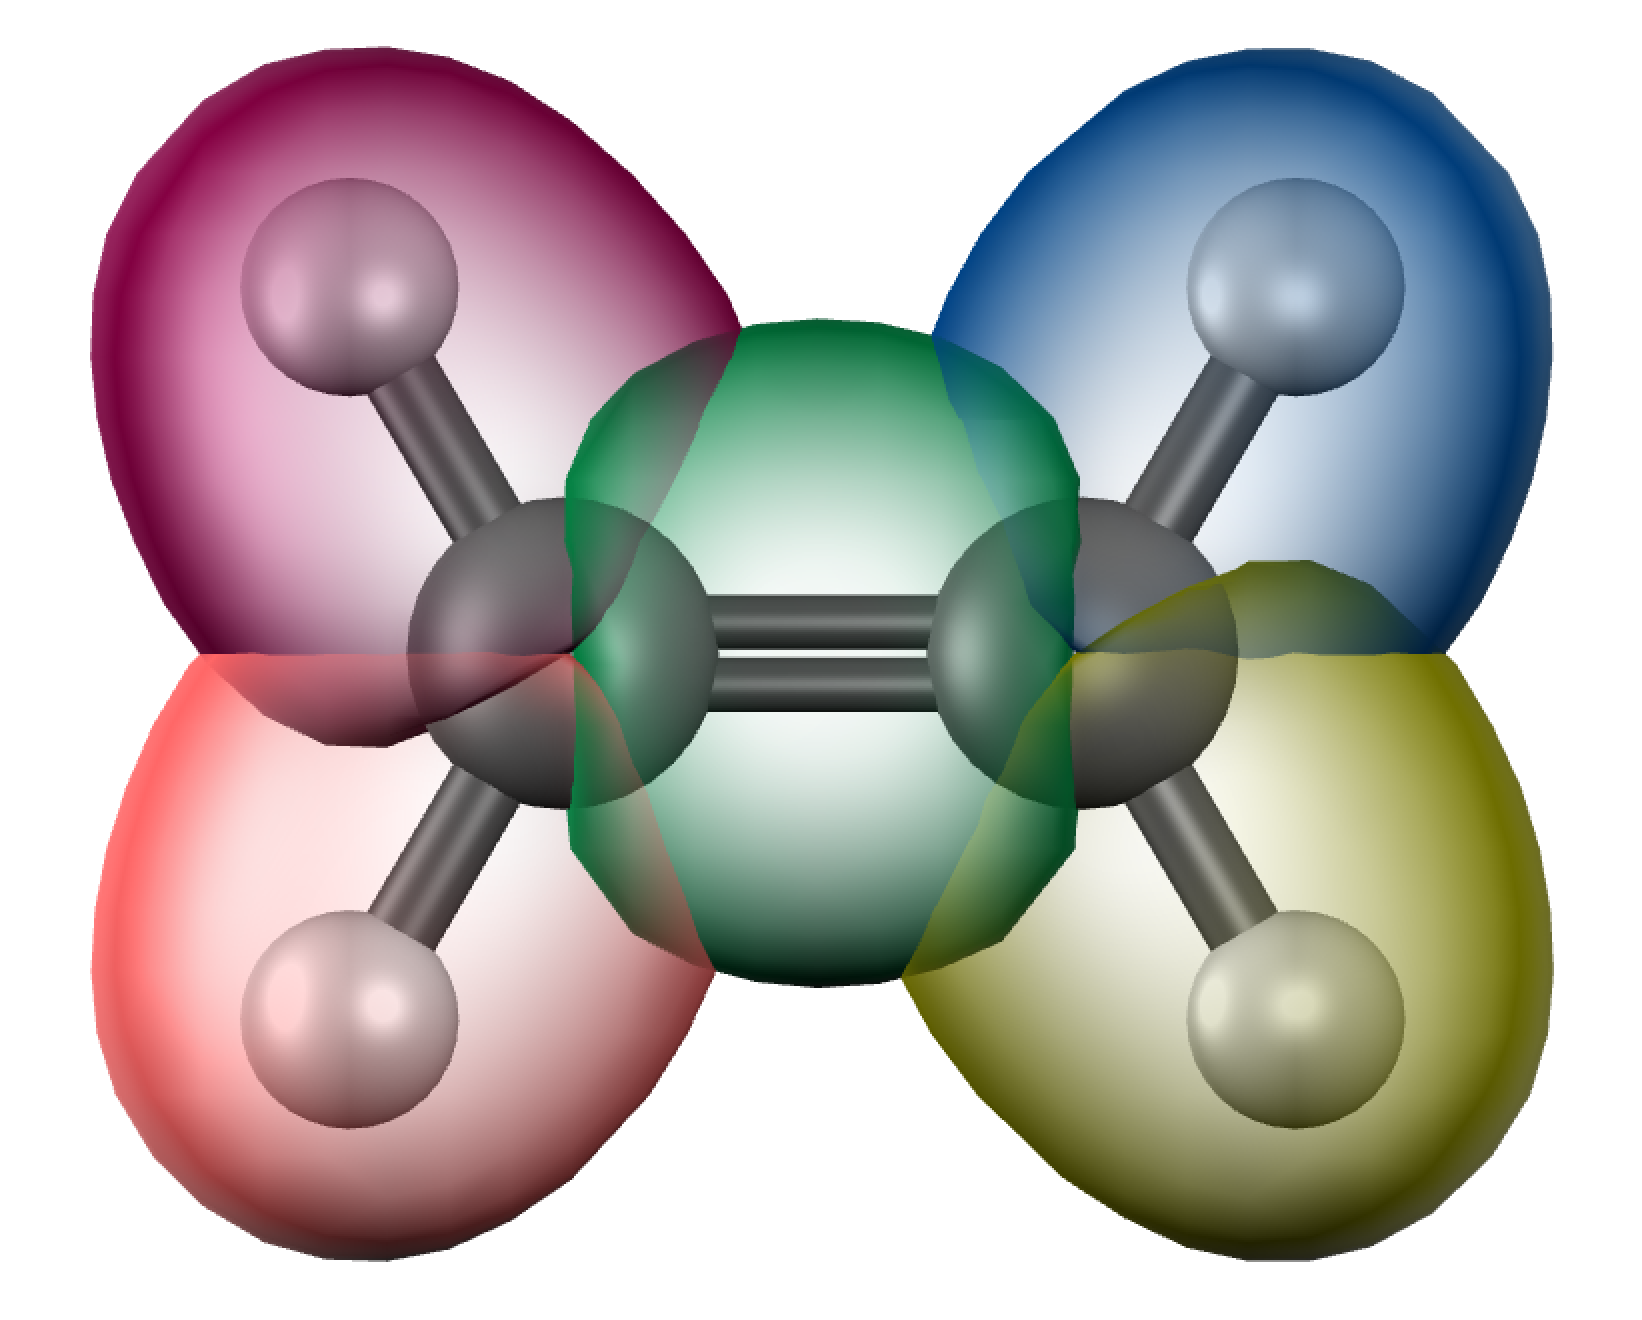
\includegraphics[scale=0.25]{figures/LocalizedBonds.png}
\caption{Localised $\sigma$-bonding orbitals in ethene.}
\label{fig:mo}
\end{center}
\end{figure}




\subsection{Exporting Cube File Data}

Each surface requires the generation of data on a 3D grid and these data are
stored internally so that subsequent calculations of the same surface (with
different isovalues, for example) are much faster.  To see what grid data is
being stored, right-click on the MO Surfaces item in the MV to bring up the
context menu.  Selecting the Show Grid Info menu brings up the Grid Information
dialog:
\begin{figure}[h]
\begin{center}
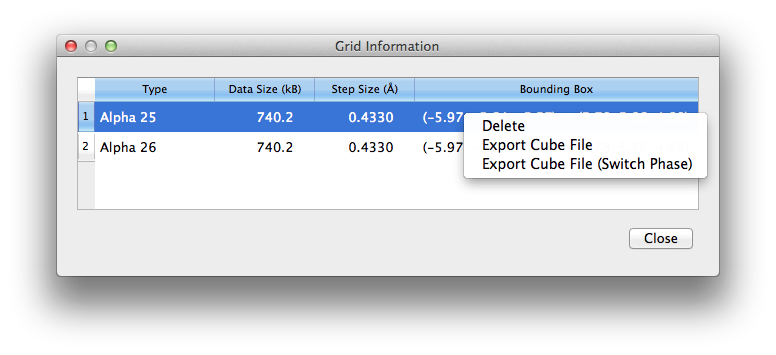
\includegraphics[scale=0.4]{figures/GridInfo.png}
\caption{The Grid Information dialog shows what data is being stored and
offers the option of exporting the data in a cube file format.}
\end{center}
\end{figure}

From this dialog it is possible to export cube files containing the grid data.
Right-clicking on the desired grid brings up a context menu with the 
Export Cube File option.  The Switch Phase option swaps the sign of the data,
and may be useful when comparing different MOs where the (arbitrary) phases
differ.  Cube files can be saved for future plotting to avoid having to
recompute the data, or for reading into another plotting package.  This is
described in the following section.


\subsection{Visualizing Cube File Data}

Cube files contain volumetric data such as electron densities, molecular
orbitals or electrostatic potentials (ESP).  Because the data has been
pre-computed, generating surfaces using them is very quick.  After opening a
cube file, a Cube Data item will appear in the MV, double-clicking this item
brings up the Add Surface dialog which allows an isovalue surface to be
requested (Fig.~\ref{fig:cubefile}).  The Signed check-box causes two
isosurfaces to be generated corresponding to $\pm$ the specified isovalue, and
this should be checked for data such as MOs and spin densities.
\begin{figure}[h]
\begin{center}
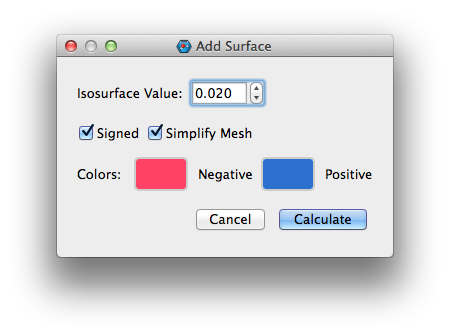
\includegraphics[scale=0.4]{figures/AddSurface.png}
\caption{The Add Surface dialog for cube data files}
\label{fig:cubefile}
\end{center}
\end{figure}

Cube file data can also be used to color a surface.  This will require either
two cube files (one containing the surface data and the second containing the
property used to color the surface) or a cube file and a checkpoint file.  In
either case, two files need to be loaded into the one molecule using the File
\bt\ Open Dir menu option, described above.

After creating a surface, double-clicking the surface item will
cause the Configure Surface dialog to appear:
\begin{figure}[h]
\begin{center}
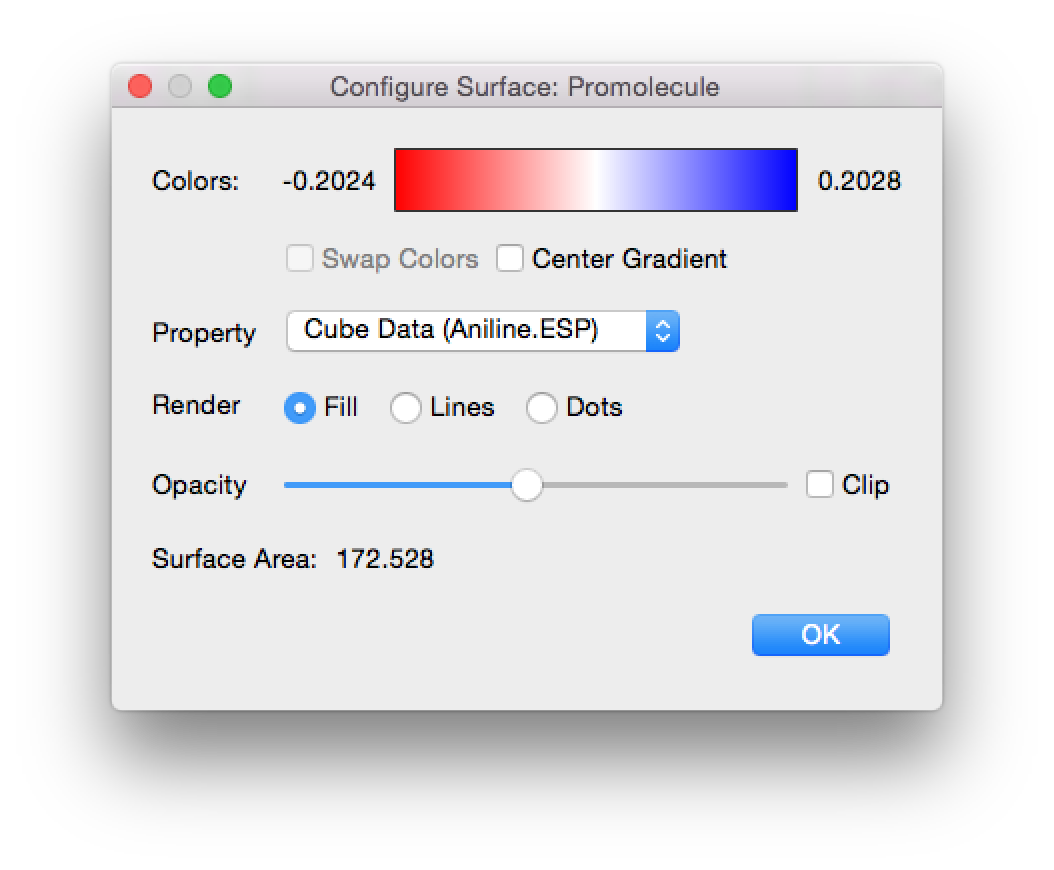
\includegraphics[scale=0.15]{figures/SurfaceConfigurator.png}
\caption{Configure Surface dialog showing the Cube Data as an option for the property.}
\label{fig:surfaceconfig}
\end{center}
\end{figure}

The Property combo-box will have the cube data as one of the options, and selecting
this will cause the surface to be colored according to the data in the cube file.
The gradient colors can be altered by clicking inside the gradient box.
\begin{figure}[h]
\begin{center}
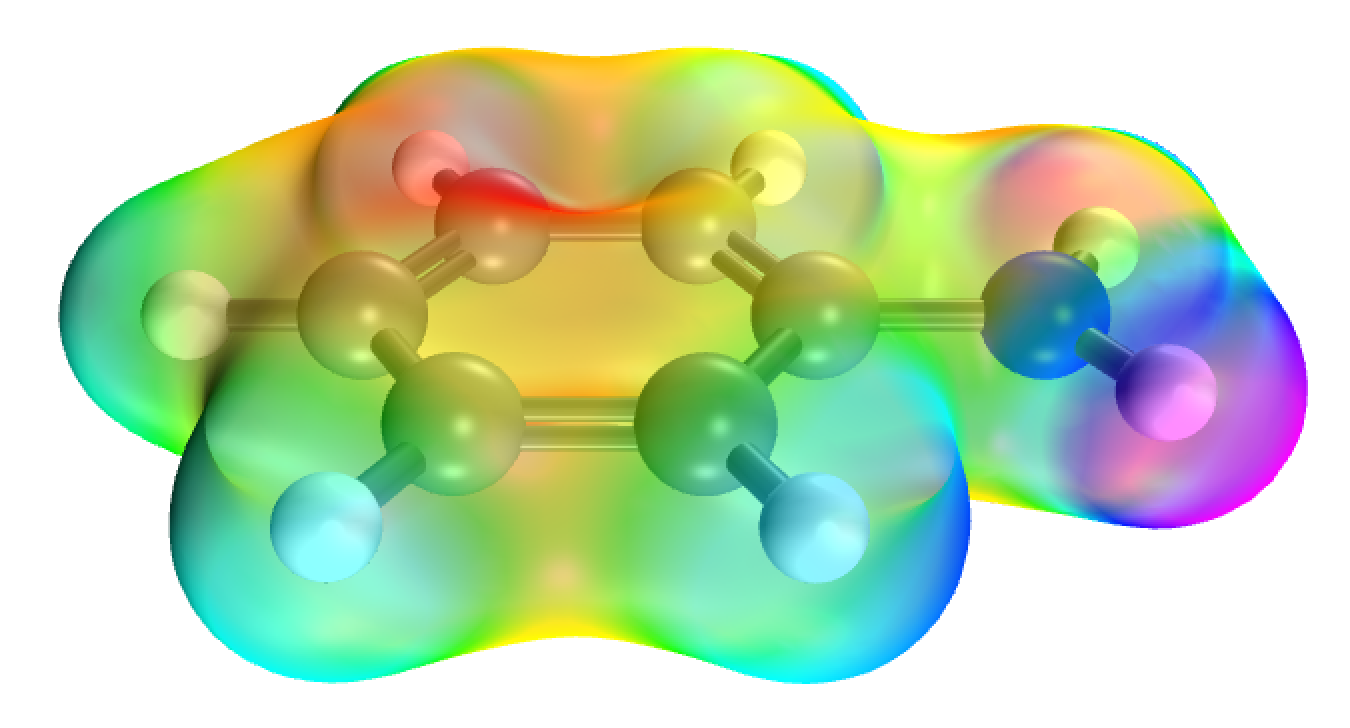
\includegraphics[scale=0.30]{figures/ESP.png}
\end{center}
\caption{Electron density plot of aniline colored according to the electrostatic potential.}
\end{figure}


\newpage
\subsection{Orbital Animations}

Orbital animations can be created \eg{}, for watching the evolution of the
frontier orbitals during a reaction, or watching the relaxation of an orbital
during a self-consistent field (SCF) calculation.  Key frames should be saved
as cube file data in a single directory.  The base name of the cube files needs
to match the directory name, \eg{}

\begin{center}
\hspace*{2em}{\tt  relaxation/relaxation.Frame.1.cube}\\
\hspace*{2em}{\tt  relaxation/relaxation.Frame.2.cube}\\
\end{center}
Open the directory, as described in Sec. \ref{sec:anal}, and right-click on the
first cube file item which appears in the MV, this will allow you to access the 
Surface Animator dialog:
\begin{center}
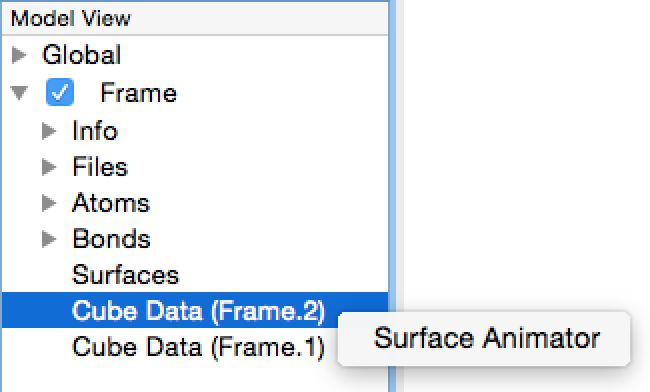
\includegraphics[scale=0.40]{figures/SurfaceAnimationMenu.png}
\end{center}
The dialog is shown in Fig. \ref{fig:SurfaceAnimationDialog} and can be used to
adjust the key frame order and the settings for the animation, including the
number of interpolation frames (higher values give smoother results, but take
longer).  Pressing \Ovalbox{Calculate} generates each frame and individual
frames can be accessed in the MV.  Use the playback options to run the
animation, recording it with the

\includegraphics[scale=0.40]{figures/RecordButton.png} button, if desired.


\begin{figure}[h]
\begin{center}
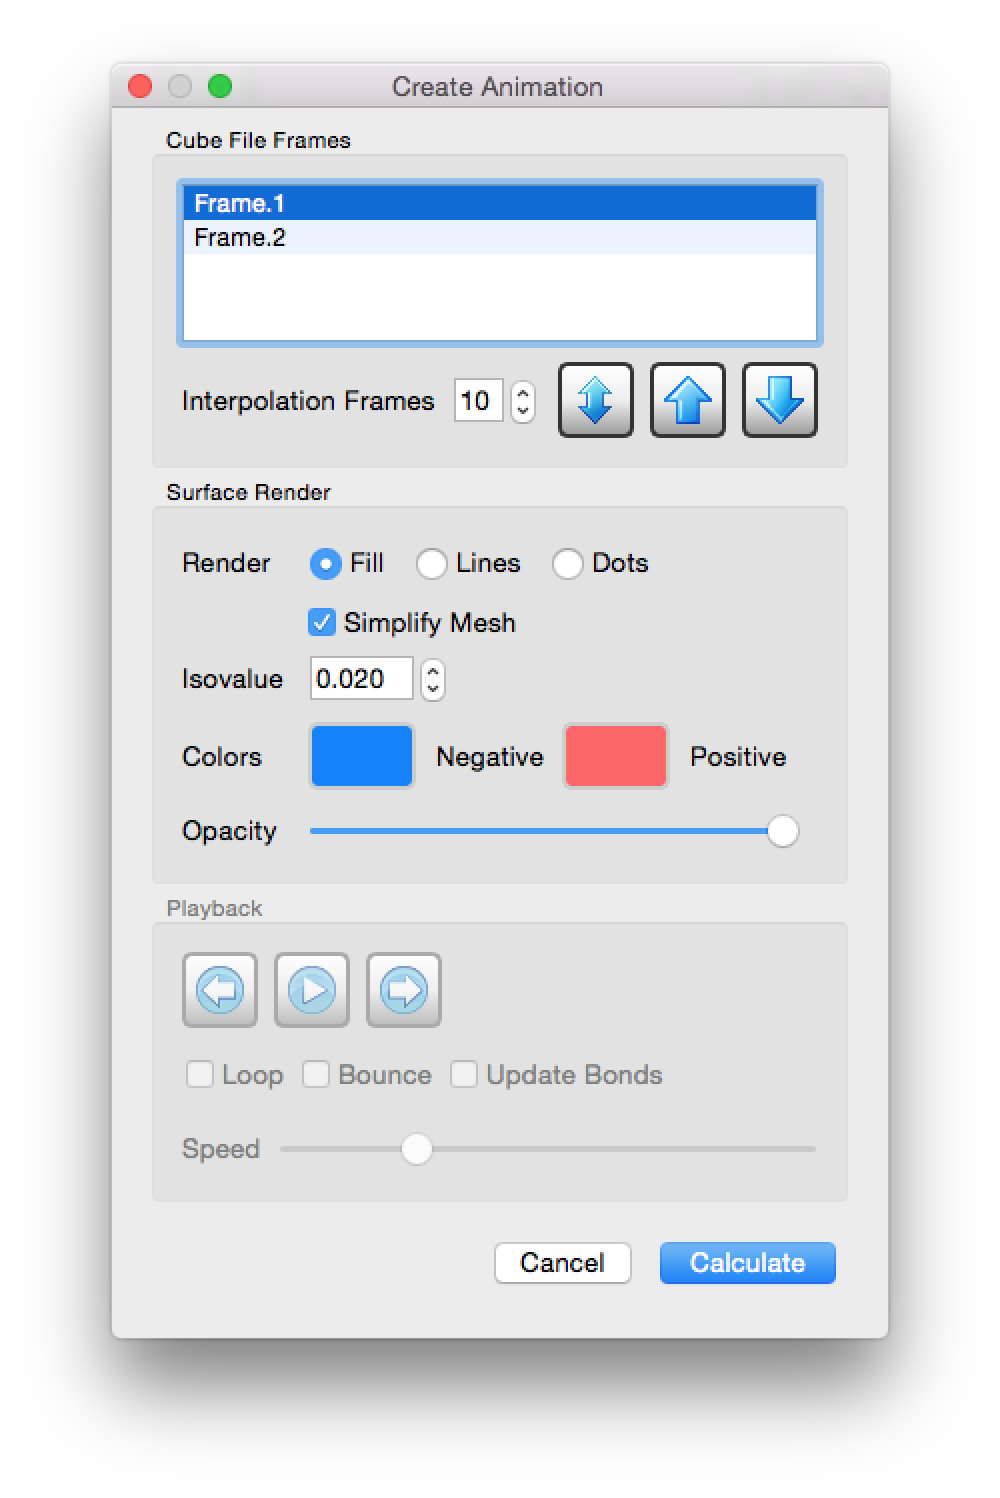
\includegraphics[scale=0.20]{figures/AnimationDialog.png}
\end{center}
\caption{The surface animation dialog.}
\label{fig:SurfaceAnimationDialog}
\end{figure}



\newpage
\subsection{Potential Energy Surfaces}

Several calculation types provide information about the potential energy
surface (PES).  These include geometry optimizations, PES scans, reaction
pathways and transition state searches.  On opening a \qchem{} output file
containing one of these job types a Geometries item appears in the MV and can
be double-clicked to bring up the Geometries dialog.
\begin{figure}[h]
\begin{center}
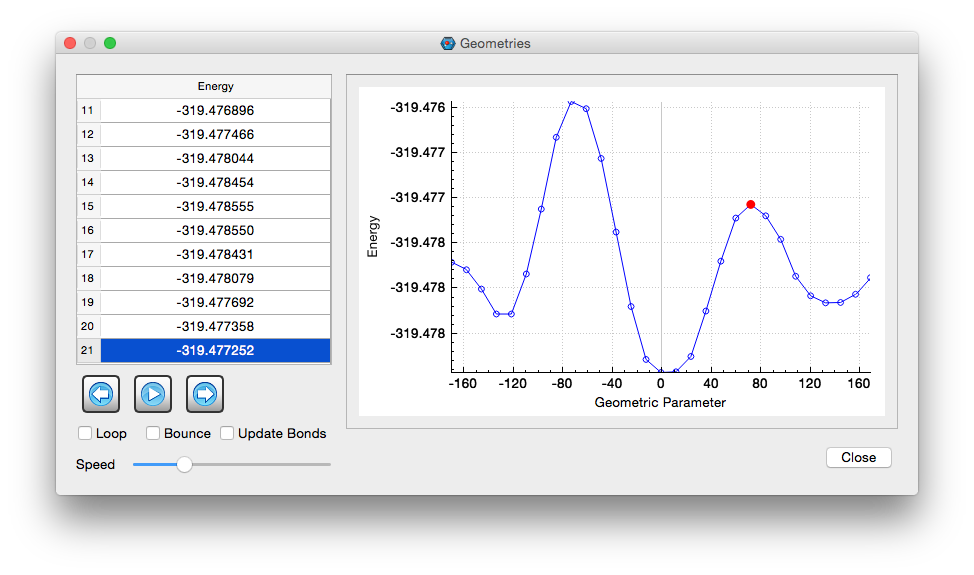
\includegraphics[scale=0.35]{figures/PesScan.png}
\caption{The Geometries dialog showing a selected geometry. }
\end{center}
\end{figure}

The pathway can be animated in the viewer using the play button, and individual
frames can be selected from either the table or by selecting a dot on the
energy plot.  The Viewer window will be automatically updated with the
corresponding structure.  As with the MO energy diagrams, the energy plot can
also be zoomed and scrolled.

Pathways can also be read in from an XYZ file.  The format for this is simply a
concatenation of regular XYZ files:
{\footnotesize
\begin{verbatim}
5
-291.77177
Si  0.71979   -0.08082   -0.76577  
H   0.73262   -1.27801    0.22990   
H   1.10451    0.93673    0.34825   
H  -1.32980    0.23894   -0.28240  
H  -1.22713    0.18317    0.47002   
5
-291.76961
Si  0.67218   -0.07483   -0.72935  
H   0.73053   -1.29428    0.22634   
H   1.10815    0.95270    0.34714   
H  -1.29502    0.23567   -0.33016  
H  -1.19409    0.17584    0.49156 
....
\end{verbatim}
}
The first line gives the number of atoms, the second (comment) line must have
the corresponding energy and then the following lines have the xyz coordinates
of each atom in the system.  This pattern repeats for as many frames as you have
available.


\subsection{Vibrational Frequencies}

Vibrational frequencies can be read in from a \qchem{} output file and appear
as a Frequencies item in the MV.  Normal mode vectors can be visualized by
selecting the associated frequency item in the MV.
\begin{figure}[h]
\begin{center}
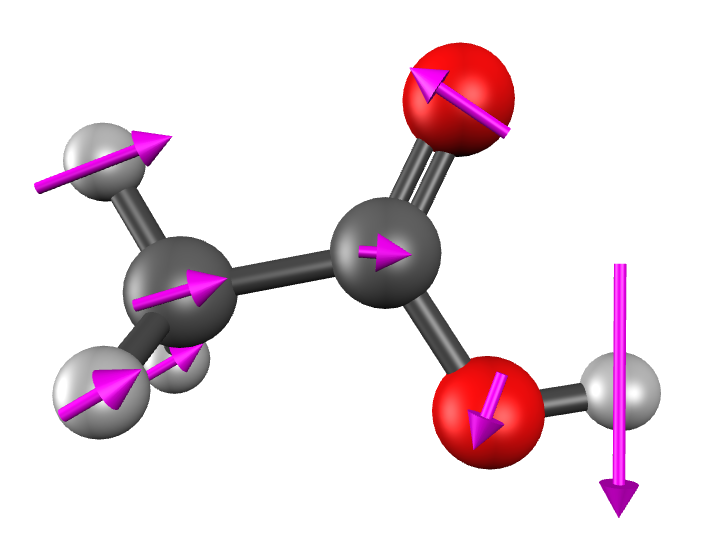
\includegraphics[scale=0.23]{figures/VibMode.png}
\caption{Arrows indicating a normal mode in acetic acid.}
\end{center}
\end{figure}

Double-clicking a frequency in the MV will cause the molecule to vibrate
according to the selected mode.  Double-clicking the Frequencies item in the 
MV will bring up the Vibrational Frequencies dialog:
\begin{figure}[h]
\begin{center}
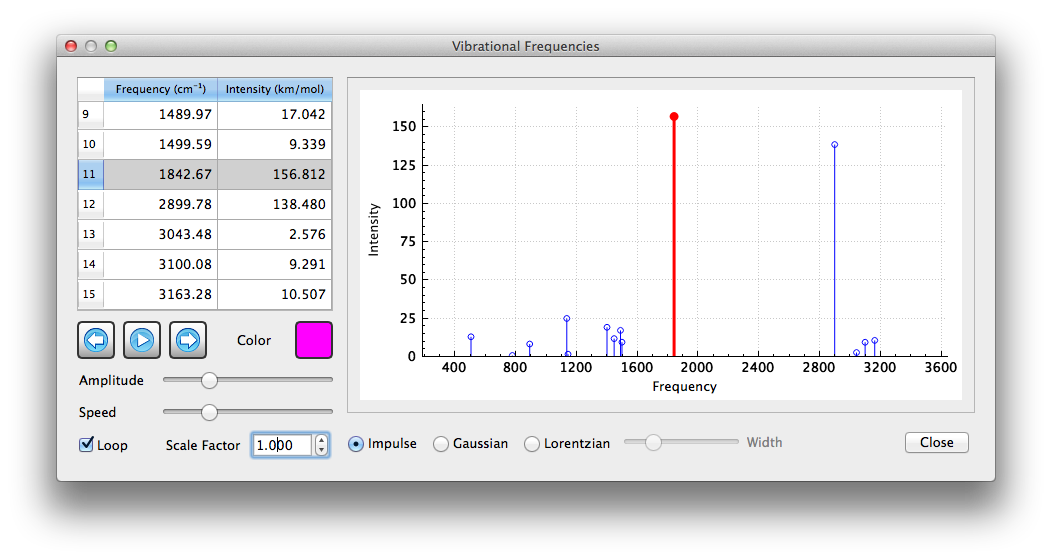
\includegraphics[scale=0.40]{figures/Frequencies.png}
\caption{The Vibrational Frequencies dialog.}
\end{center}
\end{figure}

This dialog contains an impulse spectrum showing the positions and relative
intensities of the frequencies.  Individual modes can be selected on the
spectrum by clicking the hollow circles, and this will also update the Viewer
window with the selected mode.  The impulses can be broadened using either
Gaussians or Lorentzians to give a more realistic looking spectrum, and the
image can be exported by righ-clicking on the spectrum to bring up a context
menu.

The horizontal scale of the spectrum can be zoomed (using the scroll wheel on
the mouse) and translated (left-click and drag) to give greater detail.


\subsection{NMR Spectra}

NMR shieldings and chemical shifts can be visualized using \iqmol{}.  A 
\qchem{} calculation (JOB\_TYPE = NMR) must first be run and the output
file loaded into \iqmol{}.  Shielding constants can be displayed as atom labels
in the viewer by selecting the Display \bt\ Atom Labels \bt\ NMR option.
\begin{figure}[h]
\begin{center}
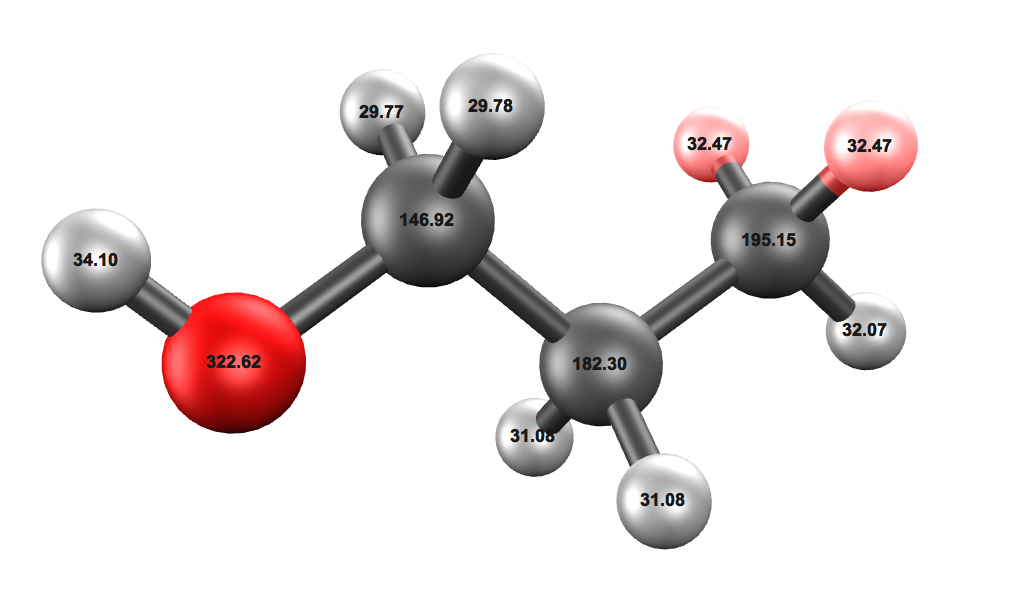
\includegraphics[scale=0.20]{figures/NmrDisplay.png}
\caption{Propanol showing the NMR shieldings}
\end{center}
\end{figure}

An NMR item will appear on in the MV and double-clicking this brings up the NMR
Spectrum dialog.
\begin{figure}[h]
\begin{center}
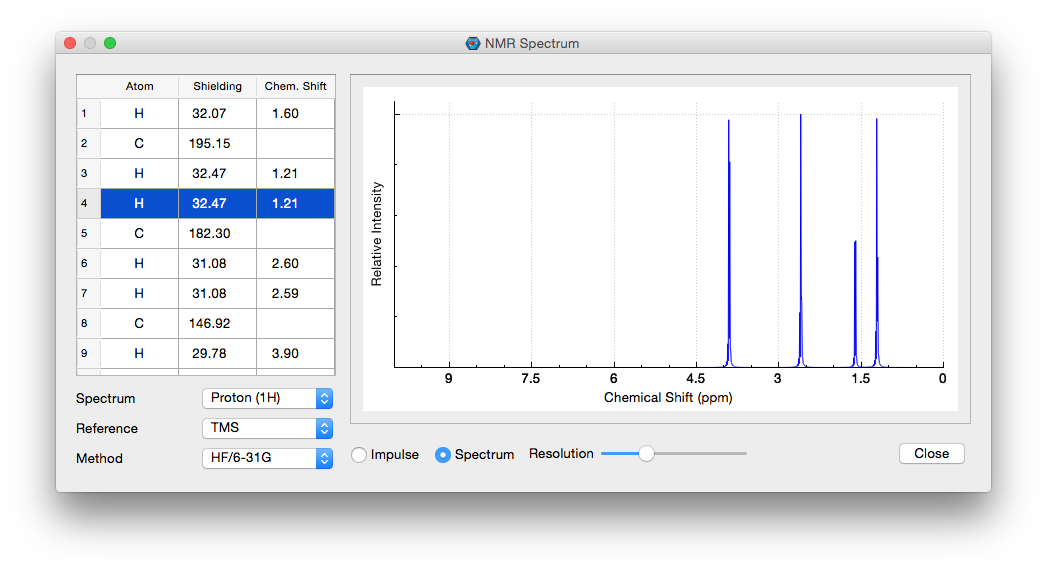
\includegraphics[scale=0.35]{figures/NmrConfigurator.png}
\caption{The NMR Spectrum dialog}
\end{center}
\end{figure}

Various spectra can be displayed ($^1$H, $^{13}$C etc.) and if 
a reference is available (\eg\ TMS) for the given level of theory, 
chemical shifts can also be displayed.  Selecting rows in the table
will also highlight the corresponding atoms in the viewer for easy
identification.  If impulses are plotted, then these can also be selected
to identify which atoms are responsible for the selected signal.

As with the vibrational frequencies spectra, NMR spectra can be exported
by right-clicking on the image to bring up the context menu.


%----------------------------------------------------------------------%
\newpage
\section{Appearance}
%----------------------------------------------------------------------%

\subsection{Viewer Camera}

When viewing a molecule, the coordinates of the atoms and surfaces are fixed in
the world reference frame.  When manipulating the molecule using the mouse (see
\S\ \ref{sec:mousemodes}) it is actually the camera that changes position and
orientation.  If more precise control of the camera is required (\eg\ for
reproducing a particular image), then the camera can be configured via the
Display \bt\ Camera menu option.  By default the camera uses a perspective
projection to give better depth perception, but an orthographic projection can
also be selected, if required.

\begin{figure}[h]
\begin{center}
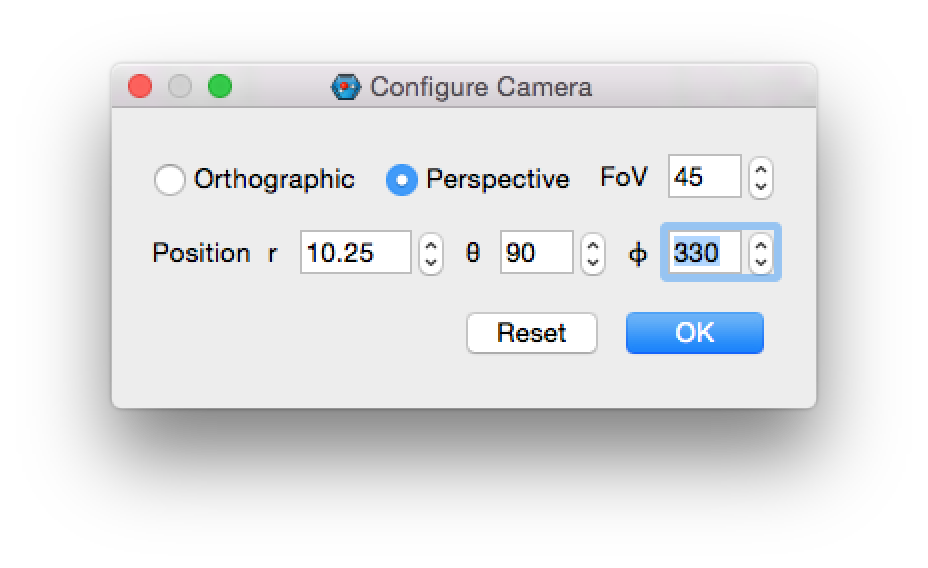
\includegraphics[scale=0.25]{figures/CameraDialog.png}
\caption{The Configure Camera dialog allows precise control over position and orientation
of the Viewer camera.}
\end{center}
\end{figure}



\subsection{Clipping Planes}

A Global clipping plane is available and can be viewed by enabling the Clipping
Plane item under Global in the MV.  Clipping planes can be useful for showing
surface information without obscuring the underlying molecular structure.
While selected, the clipping plane can be arbitrarily translated and rotated
using the manipulate selection mode described in \S\ \ref{sec:mousemodes}.
Alternatively, a precise orientation of the clipping plane can be set by
double-clicking the Clipping Plane item in the MV to open the configuration
dialog.

\begin{figure}[h]
\begin{center}
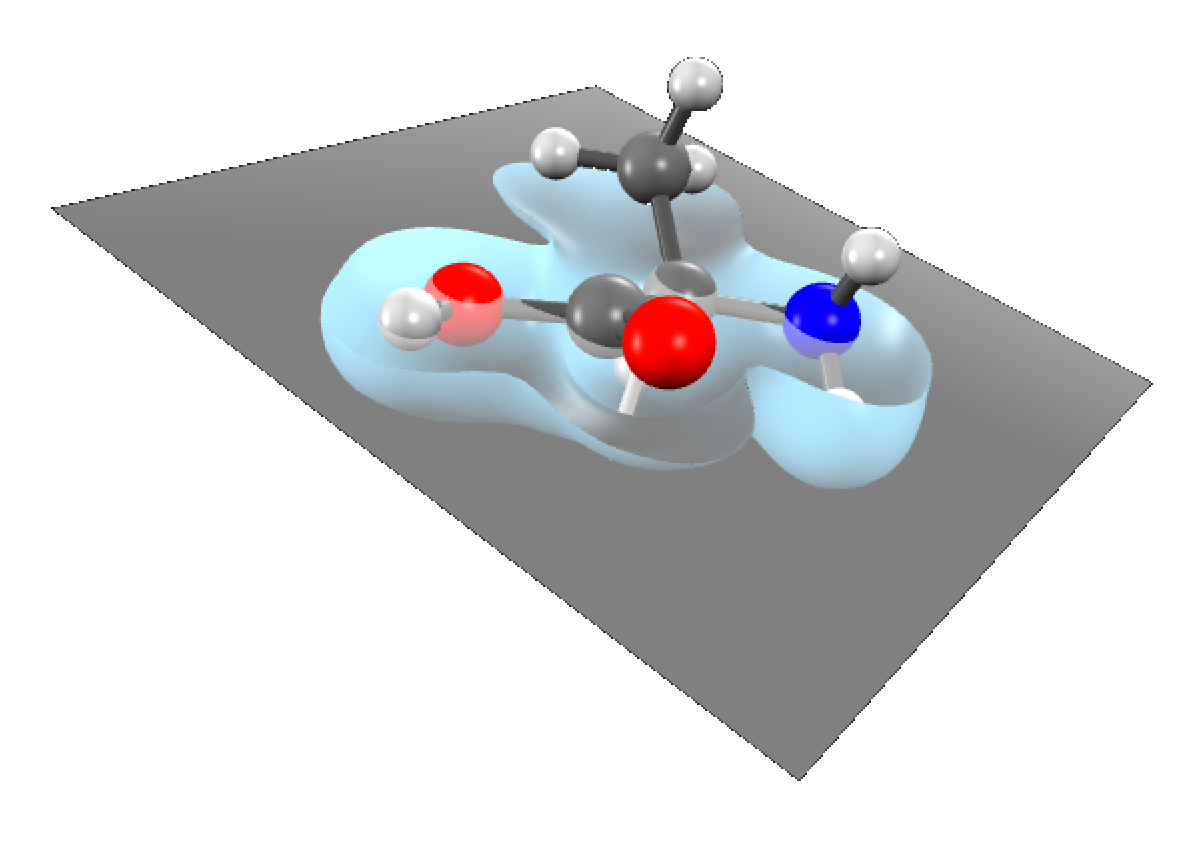
\includegraphics[scale=0.30]{figures/ClippingPlane.png}
\caption{Image showing a clipped density surface allowing the underlying
molecular structure to be more easily seen.} 
\end{center}
\end{figure}

Individual surfaces can be clipped, by selecting the Clip check-box in in the
surface configurator dialog (see Fig.~\ref{fig:surfaceconfig}) for each
surface.  Once a surface has been clipped, the clipping plane remains active
even if hidden by unchecking the Clipping Plane item check-box in the MV.


\subsection{Shaders}

\iqmol{} uses GLSL shaders to enhance the appearance of the Viewer.  Shaders can
be made active by going to the Display \bt\ Appearance menu option, and selecting
the Shader panel.
\begin{figure}[h]
\begin{center}
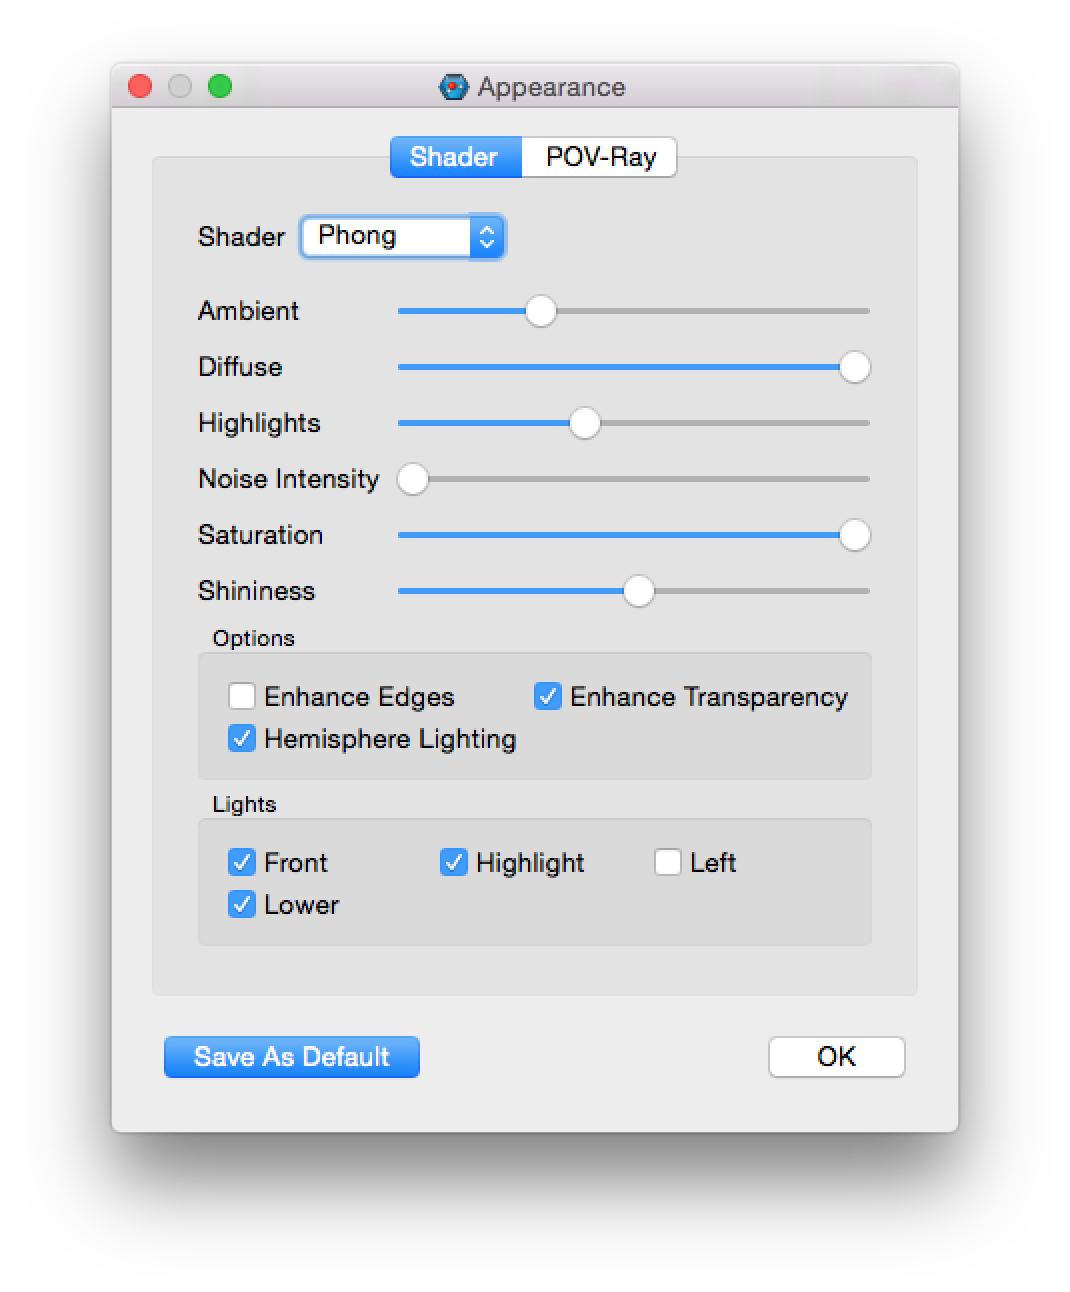
\includegraphics[scale=0.20]{figures/ShaderDialog.png}
\caption{Configuring shader options}
\end{center}
\end{figure}

Changes to the various shader options will take immediate effect and can be saved 
as the default by clicking \Ovalbox{Save As Default}.  Some shaders have several
lights associated with them, and these can be turned on or off to give different
lighting effects.


\subsection{Exporting POV-Ray Files}

\iqmol{} can generate scene files (.pov) for use with an external POV-Ray package.
POV-Ray uses ray tracing algorithms to generate images of very high quality and
resolution.  POV-Ray is open source, but several official and unofficial
packages exist with pre-compiled binaries, in particular testing was done using
the Mac version of MegaPOV.  Binaries can be downloaded from the
following sites:
\begin{itemize}
\itemsep0em
\item Mac: \url{http://megapov.inetart.net/povrayunofficial_mac}
\item Windows: \url{http://www.povray.org/download}
\end{itemize}

To export a scene file use the Edit \bt\ Generate POV-Ray Input menu option.
Scene files are plain text with instructions for the POV-Ray program, and can
be edited by the user for fine tuning before processing.  \iqmol{} can apply
several effects (\eg\ surface textures) to the molecule, and these can be
configured by opening the Appearance dialog (Display \bt\ Appearance menu
option).

\begin{figure}[h]
\begin{center}
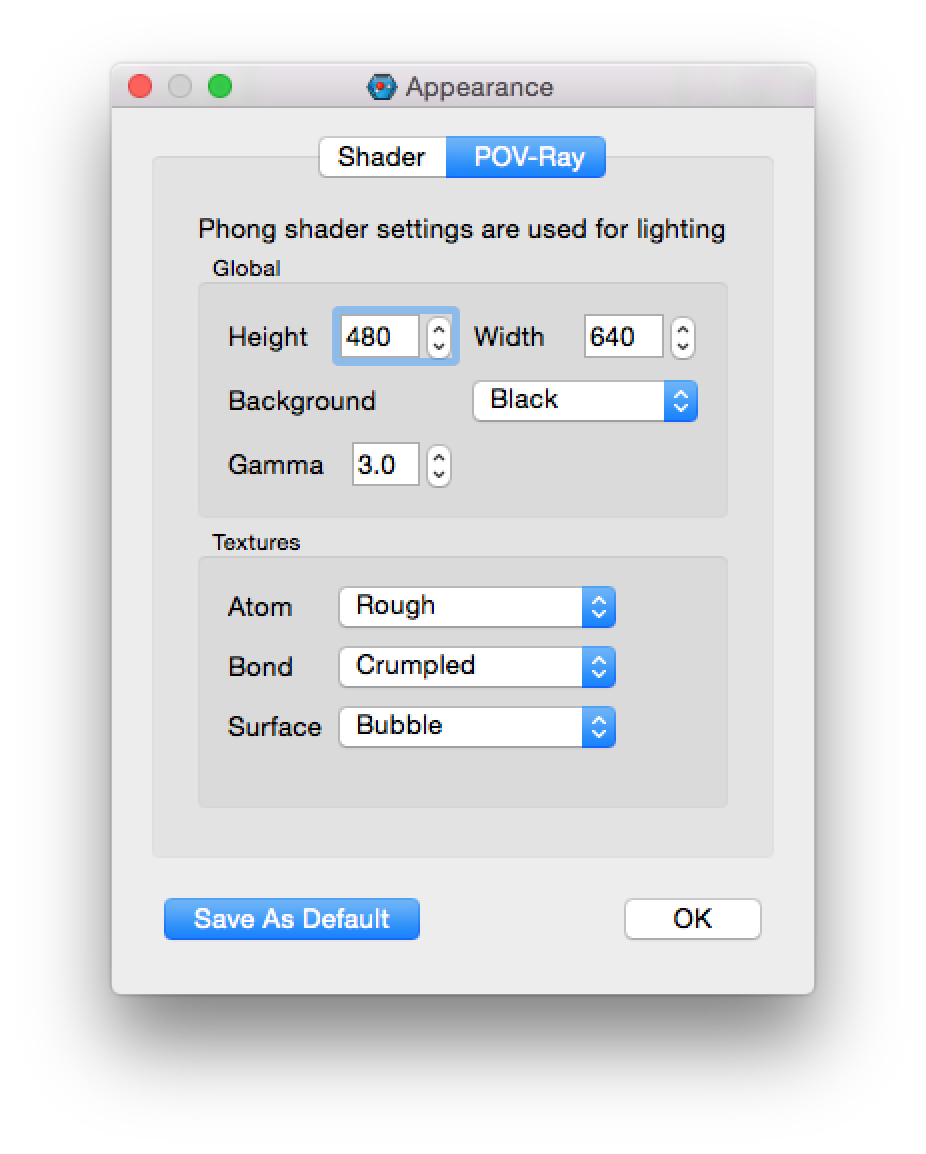
\includegraphics[scale=0.20]{figures/POVRayDialog.png}
\caption{Appearance dialog showing Options for POV-Ray scene files.}
\end{center}
\end{figure}

Note that \iqmol{} attempts to generate a scene file that matches as closely as
possible what is shown in the Viewer window.  However, there may be slight
variations in lighting, color and camera angle, and some trial and error may be
required to obtain a pleasing image.  In particular, the Gamma value may need
experimenting with, and changes to the ambient and diffuse lighting (via the
shader options) may be required depending on if a light or dark background is
selected for the scene.


%----------------------------------------------------------------------%
\newpage
\section{Sample Images}
%----------------------------------------------------------------------%

Here are some examples of the kinds of images that can be generated using
\iqmol{}'s shader and rendering options.  Most of these are simply screen
shots, however, tiles 3, 4 and 5 in the middle row were obtained by 
running POV-Ray on the \iqmol{} generated scene file.

\begin{center}
\includegraphics[scale=0.58]{figures/gallery/g13_sm.png}\
\includegraphics[scale=0.58]{figures/gallery/g14_sm.png}\
\includegraphics[scale=0.58]{figures/gallery/g15_sm.png}\
\includegraphics[scale=0.58]{figures/gallery/g16_sm.png}\
\includegraphics[scale=0.58]{figures/gallery/g21_sm.png} \\
\includegraphics[scale=0.58]{figures/gallery/g10_sm.png}\
\includegraphics[scale=0.58]{figures/gallery/g11_sm.png}\
\includegraphics[scale=0.58]{figures/gallery/g12_sm.png}\
\includegraphics[scale=0.58]{figures/gallery/g17_sm.png}\
\includegraphics[scale=0.58]{figures/gallery/g25_sm.png} \\
\includegraphics[scale=0.58]{figures/gallery/g1_sm.png}\
\includegraphics[scale=0.58]{figures/gallery/g4_sm.png}\
\includegraphics[scale=0.58]{figures/gallery/g23_sm.png}\
\includegraphics[scale=0.58]{figures/gallery/g26_sm.png}
\includegraphics[scale=0.58]{figures/gallery/g24_sm.png} \\
\includegraphics[scale=0.58]{figures/gallery/g7_sm.png}\
\includegraphics[scale=0.58]{figures/gallery/g5_sm.png}\
\includegraphics[scale=0.58]{figures/gallery/g3_sm.png}\
\includegraphics[scale=0.58]{figures/gallery/g20_sm.png}\
\includegraphics[scale=0.58]{figures/gallery/g6_sm.png} \\
\includegraphics[scale=0.58]{figures/gallery/g2_sm.png}\
\includegraphics[scale=0.58]{figures/gallery/g9_sm.png}\
\includegraphics[scale=0.58]{figures/gallery/g8_sm.png}\
\includegraphics[scale=0.58]{figures/gallery/g18_sm.png}\
\includegraphics[scale=0.58]{figures/gallery/g19_sm.png}\
\end{center}



\newpage
\bibliographystyle{acm}
\bibliography{IQmolUserGuide}


%----------------------------------------------------------------------%
\end{document}
%----------------------------------------------------------------------%

\subsection{Reaction Pathways}

\subsection{Making Movies}

\subsection{Configuration}
The Global item in the MV is always available and allows 

Preferences
appearance
Global


